\documentclass[11pt]{article}

\usepackage{graphicx}

% Enable references to labels in the notes
\usepackage{xr-hyper}
\externaldocument{p328_notes}
\usepackage{hyperref}

% Sans fonts
\usepackage{sfmath}
\renewcommand{\familydefault}{\sfdefault}

\newcommand{\COURSE}{PHYS328W}
\newcommand{\LABNUM}{8}
\newcommand{\TITLE}{Common Emitter Amplifier}
\markright{\COURSE~Lab \LABNUM\ : \TITLE}

\setlength{\textwidth} {6.5 true in}
\setlength{\textheight}{9 true in}
\setlength{\hoffset}   {-0.75 true in}
\setlength{\voffset}   {-0.75 true in}
\setlength{\parindent} {12 pt}
\pagestyle{myheadings}

\begin{document}

\thispagestyle{empty}

\section*{\COURSE\ Lab \LABNUM\ : \TITLE}

This lab relies heavily on Section~\ref{sec:commonemitter} of the notes.

\subsection*{Design}

\begin{figure}[ht]
  \begin{center}
    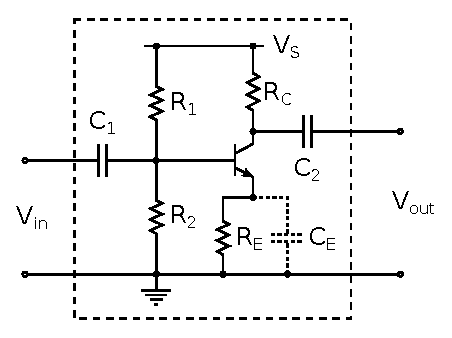
\includegraphics{commonemitter.eps}
    \caption{Schematic of an AC coupled common emitter amplifier.}
    \label{fig:commonemittercircuit}
  \end{center}
\end{figure}

Use the design process described in Section~\ref{sec:commonemitter} of
the notes to select resistors $R_1$, $R_2$, $R_E$, and $R_C$ and
coupling capacitors $C_1$ and $C_2$. Assume that we will use the
amplifier with signal frequencies above 100~Hz.

\subsection*{Simulation}

Simulate your design, and verify that it behaves as advertized. Use a
WHAT KIND OF sweep analysis to ...
\begin{enumerate}
\item Find the 3~dB point of the amplifier, and
  modify your design if it does not pass signals in the desired
  frequency range.

\item Determine the voltage gain $A_v$ of the amplifier for
  frequencies significantly above the 3~dB point, and compare your
  result with the prediction of Equation~\ref{eq:commonemittergain} of
  the notes.
\end{enumerate}



    
\subsection*{Experiment}

\begin{enumerate}
\item 
\end{enumerate}

\subsection*{Products}

Upload to Canvas a brief \LaTeX\ report in which you ...
\begin{itemize}
\item 
\end{itemize}

\end{document}
